\documentclass[psamsfonts]{amsart}

%-------Packages---------
\usepackage{amssymb,amsfonts}
\usepackage[all,arc]{xy}
\usepackage{enumerate}
\usepackage[margin=1in]{geometry}
\usepackage{amsthm}
\usepackage{theorem}
\usepackage{verbatim}
\usepackage{tikz}
\usepackage{hyperref}
\usetikzlibrary{shapes,arrows}

\newenvironment{sol}{{\bfseries Solution:}}{\qedsymbol}
\newenvironment{prob}{{\bfseries Problem:}}

\bibliographystyle{plain}

\voffset = -10pt
\headheight = 0pt
\topmargin = -20pt
\textheight = 690pt

%--------Meta Data: Fill in your info------
\title{14.27 \\
Economics of E-Commerce \\
Problem Set 2}

\author{John Wang}

\begin{document}

\maketitle

\section{Problem 3}

\begin{prob}
I will be looking at the golf ball markets on eBay. I will be searching for ``Titleist ProV1 Golf Ball New 1 Dozen'' and ``Callaway Tour Golf Ball New 1 Dozen''. Both of these searches are looking for a very specific brand of golf ball, and only for a dozen of them. The searches turned up results with more than a dozen balls, in these cases I examined the price per dozen of these balls. I wrote a python script to scrape the information from eBay's website for these golf balls.

For the Titleist balls, there were 417 listings in the past 15 days, which means that there will be roughly 800 listings of this specific product each month on eBay. Note that simply searching for ProV1 golf balls yields about $5000$ results, but these are may not necessarily be new balls still in the manufacturer's packaging. I also found another auction site \url{http://www.golfbids.net/} which was auctioning off Titlesit ProV1 balls. This auction site was more geared towards buyers who were specifically in the golf ball market. It seems that the golfbids site would be able to retain more buyers, since it seems like it attempts to form a longer term relationship with buyers and allow them to continually buy golf balls from the site. However, eBay is much easier to find on Google search (finding golfbids took a couple of minutes), so simply that may make the volume of golf ball purchases on eBay larger than the volume on golfbids. However, golfbids does have a legitimate chance of overthrowing eBay as the volume leader if they are able to credibly advertise their site, and show serious golfers that they should go back to golfbids.

\begin{figure}[h!]

\includegraphics[width=6in]{unit_price_histogram.png}
\end{figure}

The standard devition of the unit price of a dozen Titleist balls was \$8.61, with an average price of \$34.74. This standard deviation is extremely large, considering that the goods are almost identical. Examining the histogram of the prices below, we can see, however, that part of the large standard deviation is due to a couple of auctions which sold the golf balls extremely cheaply. There was a cohort of people who sold these balls for prices averaging \$10 for a dozen balls. However, even removing all products sold at prices cheaper than \$20, our new standard deviation is still \$6.95 with a mean of \$35.80. This shows that the large standard deviation is fueled both by cheap sellers, and by a large disparity of prices in general.

For the Callaway balls
\end{prob}

\section{Problem 4}

\begin{prob}
Spend a few minutes on Google Trends exploring anything your heart contents to get warmed up. Then think of a few online companies that compete with one another and compare them using both the searches and the website features. What can you infer from the data? Can you find any interesting or surprising results?
\end{prob}
\begin{sol}
I examined the trends of Amazon.com and eBay.com. Both of these companies are similar, in that they can be categorized in the online marketing and retail industry, but they differ by the types of products they sell. For instance, eBay is more of a second hand auction site, although it is moving towards an online retail business, while Amazon has much more retail business, especially in brand name products. This distinction can provide some insight into their different Google trends.

\begin{figure}[h!]
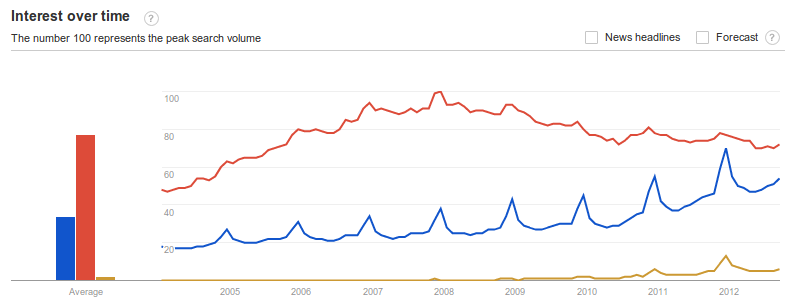
\includegraphics[width=6in]{ebay_vs_amazon.png}
\caption{eBay (Red Line) vs Amazon (Blue Line) on Google Trends}
\end{figure}

It is clear from the figure above that Amazon and eBay have completely different trends on Google searches. First, we can see that eBay seems to have reached some sort of saturation point for its growth in Google searches, whereas Amazon currently has an upward trend which is moving higher every year. This could be a reflection of the different growth phases which each company is currently in, since eBay already controls a large part of the online auction market and has few innovative products for expansion, whereas Amazon has many new technologies each year, and is pushing hard for new users. 

The other trend to notice is that Amazon is highly seasonal, whereas eBay is not. For Amazon, sales spike up without fail every December (probably due to the Christmas and Holiday season when gifts are prevalent). Ebay, however, does not perceptibly seem to be affected by seasonality. This could come from the fact that Amazon and eBay have different lines of business. In Amazon's more retail centered business, consumers usually purchase new, front-line items which were just released. Since Amazon provides a online platform for businesses to sell their latest products, consumers on Amazon are more likely to purchase gifts. However, eBay targets a set of suppliers which have an older domain of items. These are usually second hand or outdated products, which are less likely to be given as gifts. Thus, eBay sees much less of a seasonal trend, and Google searches for eBay grow much more organically.

\begin{figure}[h!]
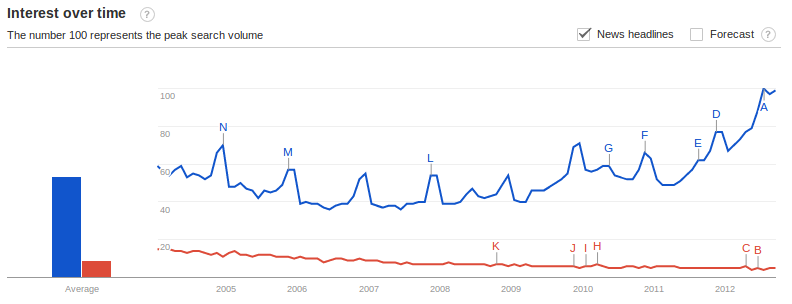
\includegraphics[width=6in]{online_shopping_vs_auction.png}
\caption{Online Auction (Red Line) vs Online Shopping (Blue Line) on Google Trends}
\end{figure}

To reinforace the hypothesis that Amazon is gaining search traction due to its business model, one can look at the Google Trends results for the terms ``Online Auction'' and ``Online Shopping''. One historically thinks of eBay as mostly an online auction site (although in recent years it has been moving to attempt to copy Amazon's model), and thinks of Amazon as a retail/shopping site. The stagnant or declining trend in people who search for ``Online Auction'' is in stark contrast to the buildup of activity in ``Online Shopping''. This last figure provides insight into why eBay and Amazon have the particular search trends that we see. These trends are correlated with the underlying business models and the type of customer that each company caters to. There has been a decline in online auctions, whereas online shopping has sped up. 
\end{sol}

\end{document}
